% !TeX root = ../tesis.tex


\chapter{Eritrocitos y sus patologías}
En este capítulo


\section{Morfología y características}
\label{section:results}

La sangre humana normal está compuesta principalmente por eritrocitos (glóbulos rojos, o RBCs por sus siglas en inglés), leucocitos, plaquetas y plasma sanguíneo \cite{mescherJunqueirasBasicHistology2024}. Este último contiene agua, electrolitos, proteínas plasmáticas, carbohidratos, lípidos y diversas vesículas extracelulares \cite{mescherJunqueirasBasicHistology2024}. Entre todos los componentes de la sangre, los eritrocitos presentan la mayor absorción óptica en el rango de 250 nm a 1100 nm, superando por dos o tres órdenes de magnitud la contribución de los otros \cite{bosschaartLiteratureReviewNovel2014a}. Por ello, constituyen el elemento dominante en las propiedades ópticas de la sangre y el principal objeto de estudio en esta sección.

\noindent Los eritrocitos son células terminalmente diferenciadas\footnote{Una célula terminalmente diferenciada se define como aquella que, al adquirir funciones especializadas, pierde  su capacidad de proliferar de manera irreversible. Por ejemplo, los eritrocitos y queratinocitos de los mamíferos, sufren una detención irreversible de su crecimiento al perder su núcleo durante la diferenciación terminal \cite{saccoCellCycleReactivation2002}.} que carecen de núcleo y están formadas casi en su totalidad por hemoglobina, la proteína responsable de sus características de absorción \cite{bosschaartLiteratureReviewNovel2014a}. La hemoglobina exhibe firmas espectrales bien definidas que dependen de su estado químico: oxihemoglobina ($\text{HbO}_2$), desoxihemoglobina (Hb), carboxihemoglobina, metahemoglobina, hemoglobina fetal, entre otros derivados \cite{bosschaartLiteratureReviewNovel2014a}. La función fisiológica principal de los eritrocitos es transportar oxígeno a través de la hemoglobina que llevan en su interior \cite{palTextbookMedicalPhysiology2021}.

\noindent En cuanto a su morfología, los eritrocitos poseen una membrana sostenida por un citoesqueleto altamente flexible que les confiere su forma característica \cite{palTextbookMedicalPhysiology2021}. Presentan un contorno ovalado y un diámetro promedio de aproximadamente 7.5 $\mu$m. Su geometría incluye una depresión central que reduce el espesor en la región media, dando lugar a un disco bicóncavo con un grosor de alrededor de 2.6 $\mu$m en los bordes y aproximadamente 0.75 $\mu$m en el centro \cite{palTextbookMedicalPhysiology2021}, como se muestra en las Figs. \ref{fig:erythrocytes}. Esta estructura no solo es esencial para su función fisiológica, al proporcionar una gran relación superficie-volumen y facilitar el intercambio de gases \cite{palTextbookMedicalPhysiology2021}, sino que también influye directamente en su comportamiento óptico y en la manera en que esparcen la luz \cite{bosschaartLiteratureReviewNovel2014a}.

\begin{figure}[t]
	\centering
	\sidesubfloat[First image]{
	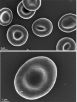
\includegraphics[width=0.3\textwidth]{../Figuras/SEM_erythrocyte.pdf}\label{subfig:SEM}}\hspace{0.5cm}
	\sidesubfloat[Second image]{	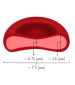
\includegraphics[width=0.35\textwidth]{../Figuras/erythrocyte.pdf}\label{subfig:ery}}
	\caption{Estructura de un eritrocito sano. \textbf{a)} Micrografías electrónicas de barrido (SEM por sus siglas en inglés) de eritrocitos de pacientes sanos. La micrografía superior muestra eritrocitos de forma bicóncava normal con interacción limitada, mientras que la inferior muestra un eritrocito sano con una membrana ligeramente granular; imágenes extraídas y adaptadas de \cite{alummoottilScanningElectronAtomic2023}. \textbf{b)} Diagrama de un corte longitudinal de un eritrocito que muestra las dimensiones de la célula. }
	\label{fig:erythrocytes}
\end{figure}